% !TEX root = main.tex
% ======================================================================
%  BIBM / IEEE 课程论文模板（支持中英文混排）
%  适用课程：《生物文本挖掘与知识发现》
%  最终稿：文献获取、词汇统计、实体归一化、SDP 关系抽取与知识验证
%  作者：易子茗（2024317240212，生信2402）
%  编译方式：xelatex -> bibtex -> xelatex -> xelatex
% ======================================================================
\documentclass[conference]{IEEEtran}
\IEEEoverridecommandlockouts

% ---------- 基础宏包 ----------
\usepackage{cite}
\usepackage{amsmath,amssymb,amsfonts}
\usepackage{algorithmic}
\usepackage{graphicx}
\usepackage{textcomp}
\usepackage{xcolor}
\usepackage{url}
\usepackage{booktabs}
\usepackage{tabularx}
\usepackage{multirow}

% ---------- 双栏浮动体参数 ----------
\setcounter{dbltopnumber}{2}
\renewcommand{\dbltopfraction}{0.90}
\renewcommand{\dblfloatpagefraction}{0.80}
\setlength{\dbltextfloatsep}{5pt plus 1pt minus 1pt}
\setlength{\textfloatsep}{5pt plus 1pt minus 1pt}
\setlength{\floatsep}{5pt plus 1pt minus 1pt}
\setlength{\dblfloatsep}{5pt plus 1pt minus 1pt}

% ---------- 页码与页脚 ----------
\usepackage{fancyhdr}
\pagestyle{fancy}
\fancyhf{}
\fancyfoot[C]{\thepage}
\renewcommand{\headrulewidth}{0pt}
\renewcommand{\footrulewidth}{0pt}

% ---------- 页脚左下角灰色水印（模板要求，必须展示） ----------
\fancyfoot[L]{%
  \scriptsize\color{gray}%
  \begin{tabular}[b]{@{}l@{}}
    课程论文支持使用 Agent 生成内容，\\
    这只是起点。人工内容审查\\
    和驾驭才是终点。%
  \end{tabular}%
}
\setlength{\footskip}{24pt}

% IEEEtran 首页 \maketitle 默认使用 plain / IEEEtitlepagestyle，需同步页脚
\fancypagestyle{plain}{%
  \fancyhf{}%
  \fancyfoot[C]{\thepage}%
  \fancyfoot[L]{%
    \scriptsize\color{gray}%
    \begin{tabular}[b]{@{}l@{}}
      课程论文支持使用 Agent 生成内容，\\
      这只是开始。人工内容审查\\
      和驾驭才是终点。%
    \end{tabular}%
  }%
  \renewcommand{\headrulewidth}{0pt}%
  \renewcommand{\footrulewidth}{0pt}%
}
\fancypagestyle{IEEEtitlepagestyle}{%
  \fancyhf{}%
  \fancyfoot[C]{\thepage}%
  \fancyfoot[L]{%
    \scriptsize\color{gray}%
    \begin{tabular}[b]{@{}l@{}}
      课程论文支持使用 Agent 生成内容，\\
      这只是开始。人工内容审查\\
      和驾驭才是终点。%
    \end{tabular}%
  }%
  \renewcommand{\headrulewidth}{0pt}%
  \renewcommand{\footrulewidth}{0pt}%
}

% ---------- 行号 ----------
\usepackage[switch]{lineno}
\pagewiselinenumbers

% ---------- 中文支持 ----------
\usepackage[UTF8]{ctex}
\setmainfont{Times New Roman}

\def\BibTeX{{\rm B\kern-.05em{\sc i\kern-.025em b}\kern-.08em
    T\kern-.1667em\lower.7ex\hbox{E}\kern-.125emX}}

\begin{document}

\title{基于PubMed文献挖掘与水稻性状本体的\\水稻抗旱基因-性状关联知识发现}

\author{
\IEEEauthorblockN{易子茗}
\IEEEauthorblockA{
\textit{2024317240212} \\
\textit{华中农业大学信息学院} \\
代码仓库: \url{https://github.com/ZimingADR/BioNLP}}
}

\maketitle

\begin{abstract}
水稻抗旱知识散落在海量非结构化文献中，通用生物医学 NER 又缺乏作物性状维度。本文构建了一条从 PubMed 语料到可复核知识图谱的端到端流水线：检索并解析 3,306 篇抗旱文献（35,345 句、795,401 词元），融合 Oryzabase 的 102,860 条基因别名与 RTO-1.0 的 3,904 条性状同义词，经五重农学消歧获得 10,708 个 RAP 归一化基因提及与 29,966 个性状提及，形成 7,868 条水稻候选共现对。在此基础上，本文用 spaCy 依存句法树提取最短依存路径（SDP），结合论元角色、调控谓词、否定与 \texttt{respectively} 对齐，将候选压缩为 884 条因果调控关系（575 正、150 负、159 中性）与 1,379 条 association。100 条分层人工审计显示 SDP precision 达 86.0\%（95\% CI 73.8--93.0），显著高于共现基线的 34.5\%，极性判别准确率 88.2\%；TO/RTO 富集得到 53 个显著条目，RiceMind 覆盖 99\% 的 Top100 基因并暴露 13 个抗逆注释缺口候选。本文为作物抗逆知识图谱提供了高保真、可追溯的语料与关系底座。
\end{abstract}

\begin{IEEEkeywords}
生物自然语言处理, 水稻抗旱性, 最短依存路径, 水稻性状本体, 知识图谱
\end{IEEEkeywords}

\section{引言}
水稻（\textit{Oryza sativa} L.）是全球半数以上人口的主粮，其抗逆稳产是气候变化下保障粮食安全的关键。过去二十年，ABA 信号、渗透调节、根系构型等方向克隆了大量抗旱基因，但“基因--表型”证据仍以自由文本散落在数千篇 PubMed 摘要中，人工汇总耗时且易漏。

将通用 BioNLP 模型迁移到作物领域面临三重偏移：(1) 检索歧义：\texttt{rice} 既是水稻俗名，也是姓氏与校名，单一短语易漏检或误检；(2) 表型缺位：PubTator 等医学 NER 不识别 \texttt{drought tolerance}、\texttt{leaf rolling} 等农艺性状 \cite{wei2024pubtator3}；(3) 命名异构：同一基因在不同论文中写作 \texttt{SNAC1}、\texttt{OsNAC9}、\texttt{ONAC2}，而 \texttt{ABA}、\texttt{ha-1} 等生理缩写又与冷门突变体别名冲突。此外，句子级共现并不等于因果，否定句与 \texttt{respectively} 并列句会制造大量假阳性。

针对上述问题，本文完成了一条四阶段流水线，贡献如下：
\begin{enumerate}\setlength{\itemsep}{0pt}\setlength{\parsep}{0pt}\setlength{\topsep}{1pt}
  \item \textbf{高召回、低歧义语料构建}：以双名法、MeSH 与标题/摘要字段约束检索式，严格遵守校园网限流（\texttt{sleep 5.8s}），获得 3,306 篇 PubTator 全文，35,345 句、795,401 词元。
  \item \textbf{词汇计量与检索反证}：用 Heaps' Law 与多尺度 TTR 解释词汇稀释，用 TF-IDF 二元短语证明 \texttt{drought stress} 相对 \texttt{drought tolerance} 多覆盖 41.9\% 文献。
  \item \textbf{双词典五重消歧与共现基线}：融合 Oryzabase 与 RTO-1.0，建立 102,860 条基因别名与 3,904 条性状同义词；在 7,868 条水稻候选对上获得 4,678 个唯一基因-性状对。
  \item \textbf{SDP 因果抽取与知识验证}：spaCy 依存树 + 论元模式 + 极性/否定/并列消歧，得到 884 条因果调控关系；100 条人工审计 precision 86.0\%，并完成 TO/RTO 富集与 RiceMind 注释缺口分析。
\end{enumerate}

\section{相关工作}
生物医学文本挖掘已从词典/规则走向深度学习。Cancer-Alterome 通过文献检索、词典标注与依存抽取构建癌症调控事件资源 \cite{canceralterome2024}；PubTator 3.0 提供在线实体预标注 \cite{wei2024pubtator3}；NLTK 提供稳定的英文分句与分词接口 \cite{nltk2009}。课程讲义系统给出了 PubTator 字符偏移与 NLTK 句子边界对齐、句子级证据表构建的规范 \cite{slides2026}。

在稻作知识库方面，Oryzabase 与 RAP-DB 汇集了 CGSNL 标准符号、历史别名与 RAP 位点编号 \cite{kurata2006oryzabase,sakai2013rapdb}；RiceMind 提供文献挖掘的基因-性状关联与多组学注释 \cite{ricemind2024}；RTO-1.0 为水稻农艺与逆境表型建立层次化术语体系 \cite{rto2026}。关系抽取方面，基于依存句法树的最短路径（SDP）是生物事件抽取的经典范式 \cite{fundel2007}；功能验证常用超几何富集与 BH 校正 \cite{ashburner2000,huang2009}。本文把上述资源耦合为一条可审计的流水线，并重点解决农业实体归一化与共现假阳性两个领域瓶颈。

\section{数据与方法}

\subsection{数据获取与限流}
检索式限定标题/摘要/MeSH，兼顾拉丁学名与俗名，并排除作者姓氏与机构歧义：
{\centering\vspace{-2pt}\small\ttfamily ("Oryza sativa"[Title/Abstract] OR "Oryza sativa"[MeSH Terms] OR "rice"[Title/Abstract]) AND "drought"[Title/Abstract]\par\vspace{-2pt}}

该式命中 3,311 篇；通过 PubTator \texttt{export/pubtator} 接口按单篇循环下载，每篇强制 \texttt{time.sleep(5.8)}，并提供断点续传批量模式。除 5 篇 2026 年新上线文献尚未被 PubTator 索引外，其余 3,306 篇全部成功解析，构成全量语料。

\subsection{词典构建与五重农学消歧}
PubTator 记录由标题行、摘要行与实体行组成。按讲义规范拼接 \texttt{text = title + " " + abstract}，确保字符偏移 $[b,e)$ 与切片 \texttt{text[b:e]} 严格对齐。

RTO-1.0 解析全部 \texttt{[Term]} 节点，过滤 \texttt{is\_obsolete} 与顶层抽象词，提取标准名与同义词，得到 2,022 个标准性状节点、3,904 条可匹配同义词（如 \texttt{drought resistance} 与 \texttt{drought tolerance} 统一到 \texttt{TO:0000276}）。Oryzabase 解析 22,023 条基因记录，以 RAP ID 为第一标识，缺失时回退 Oryzabase ID；拆解 CGSNL 符号与同义词字段时执行五类规则：
\begin{itemize}\setlength{\itemsep}{0pt}\setlength{\parsep}{0pt}\setlength{\topsep}{0.5pt}
  \item \textit{缺省占位符回退}：首列为 \texttt{\_} 的 6,000 余条基因，剔除占位符并回退首个有效同义词；
  \item \textit{暂定名剥离}：正则 \texttt{\textbackslash(t\textbackslash)\textbackslash*?} 剥离 \texttt{Hd6(t)*} 中的 \texttt{t}，避免单字母别名污染；
  \item \textit{激素/生理缩写黑名单}：拦截 \texttt{ABA}、\texttt{AsA}、\texttt{JA}、\texttt{ROS}、\texttt{MDA}、\texttt{CAT}、\texttt{SOD} 等与突变体同形的缩写；
  \item \textit{育种世代与泛家族名}：拦截 \texttt{M1}--\texttt{M5}、\texttt{BC1}、\texttt{B2}、\texttt{B3} 及单独出现的 \texttt{MYB}、\texttt{WRKY}、\texttt{NAC}；
  \item \textit{产量单位与品种名}：拦截 \texttt{t ha-1} 中的 \texttt{ha-1}（与 \texttt{AHA8} 别名冲突）及对照品种 \texttt{Apo}（与穗型基因 \texttt{APO} 冲突）。
\end{itemize}
最终得到 102,860 条高纯度基因别名映射。

\subsection{词汇计量与句子级共现}
设小写词元序列 $W=(w_1,\dots,w_N)$，独立词型集合 $V(W)$，原始 $\text{TTR}=|V(W)|/N$。受 Heaps 定律 $|V(N)|\approx K N^{\beta}$ 支配，TTR 随长度幂律衰减。为消除长度稀释与单篇主题聚集，在固定窗口 $k\in\{10^3,5\times10^3,10^4,5\times10^4,10^5,5\times10^5\}$ 下对比顺序截断 $\text{TTR}_{\text{head}}(k)$ 与 $M=10$ 次全局随机抽样均值 $\text{TTR}_{\text{shuf}}(k)$：
\begin{equation}
\begin{aligned}
\text{TTR}_{\text{head}}(k) &= \frac{|V(w_{1:k})|}{k}, \\
\text{TTR}_{\text{shuf}}(k) &= \frac{1}{M}\sum_{m=1}^{M}\frac{|V(\mathcal{S}_m(W,k))|}{k}.
\end{aligned}
\label{eq:ttr}
\end{equation}

对候选词元/二元短语 $t$（要求 $DF(t)\ge\max(2,0.005|D|)$）计算平滑 IDF 与全语料累计 TF-IDF：
\begin{equation}
\begin{aligned}
IDF(t) &= \ln\!\left(\frac{1+|D|}{1+DF(t)}\right)+1,\\
\text{Score}(t) &= \sum_{d\in D}\frac{f_{t,d}}{|d|}\cdot IDF(t).
\end{aligned}
\label{eq:tfidf}
\end{equation}

句子级证据严格复用讲义第 51 页的 \texttt{sentence\_spans(text)}，得到句子的字符跨度 $[b_{s_i},e_{s_i})$。句内采用 $k=4\to1$ 最长匹配优先扫描，命中基因/性状词典且未被 PubTator 非基因实体掩码占用时，记录绝对坐标并断言 \texttt{text[b:e]==mention}。同一句同时含至少一个 RAP 归一化基因与一个 RTO 性状时，输出候选共现对。仅保留 RAP ID 以 \texttt{Os} 开头的水稻基因，最终得到 7,868 条候选（4,678 个唯一对）。

\subsection{基于最短依存路径的因果抽取}
对每个候选句用 spaCy \texttt{en\_core\_web\_sm} 构建依存树，将实体字符跨度映射为 token span，并取名词短语中心词。在依存图上求基因中心词与性状中心词的最短路径 $P=(u_0,\dots,u_L)$，$L$ 为路径边数。沿 $P$ 及其支配动词选择调控谓词 $v$，要求满足以下任一论元模式：
\begin{itemize}\setlength{\itemsep}{0pt}\setlength{\parsep}{0pt}\setlength{\topsep}{0.5pt}
  \item \textbf{主动}：基因位于 $v$ 的 \texttt{nsubj}/\texttt{nsubjpass} 子树，性状位于 \texttt{dobj}/\texttt{attr} 或 \texttt{to/of/for} 介词宾语；
  \item \textbf{被动}：性状为 \texttt{nsubjpass}，基因位于 \texttt{by}-agent；
  \item \textbf{名词化}：\texttt{overexpression/knockout of GENE} 作主语，性状作宾语；
  \item \textbf{链式}：$v_1$ 的主语含基因，$v_2$ 的宾语为性状，且 $v_2$ 位于 $v_1$ 的补足语/关系从句子树（如 \textit{has the potential to improve}）。
\end{itemize}

极性由谓词词典（positive/negative/neutral）、否定词与程度副词共同判定；若主语含 loss-of-function 构建（knockout、silencing、mutation、inactivation、repression 等），则对谓词极性取反，从而把“knockout 降低 tolerance”还原为“gene 正向调控 tolerance”。对含 \texttt{respectively} 的句子，按基因/性状出现顺序建立配对，索引不一致的候选标记为 \texttt{excluded\_respectively}。最终关系分为 positive/negative/regulation 三类因果、association、no\_effect 与 excluded；按路径长度、论元模式和极性明确度给出 high/medium/low 置信度。

\subsection{富集验证与 RiceMind 交叉比对}
以 SDP 因果基因集为查询集 $Q$（$|Q|=k$），在 RiceMind+文献构建的背景基因库 $B$（$|B|=N=2{,}218$）中，对每个 TO/RTO 条目 $T_j$ 统计背景命中数 $m_j$ 与查询命中数 $x_j$，计算超几何上尾概率并用 BH 校正：
\begin{equation}
p_j=\Pr(X\ge x_j\mid N,m_j,k)=\sum_{i=x_j}^{\min(m_j,k)}
\frac{\binom{m_j}{i}\binom{N-m_j}{k-i}}{\binom{N}{k}}.
\label{eq:hyper}
\end{equation}
同时调用 RiceMind \texttt{gene-profile} 接口，对 Top100 因果基因统计数据库覆盖率、\texttt{trait\_class}/\texttt{annotation} 中 stress/drought 注释比例，并把“SDP 证据 $\ge3$ 个唯一对但 RiceMind 无 stress 注释”的基因列为注释缺口候选。

\section{结果}

\begin{figure*}[t]
  \centering
  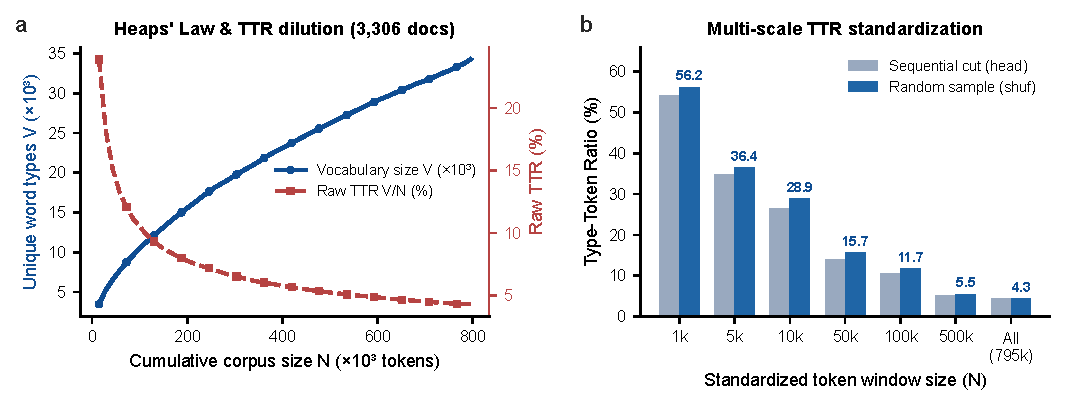
\includegraphics[width=0.63\textwidth]{figure/fig1_ttr_heaps.pdf}
  \caption{3,306 篇文献（795,401 词元）的词汇增长与多尺度 TTR。(a) Heaps 定律与原始 TTR 稀释；(b) 固定窗口下顺序截断（head）与 10 次全局随机抽样（shuf）的 TTR 对比。}
  \label{fig:ttr}
\end{figure*}

\subsection{语料与词汇计量}
全量语料共 35,345 句（平均每篇 10.69 句）、795,401 词元、34,247 个独立词型；PubTator 原生 47,157 个实体中 47,156 个通过 \texttt{text[b:e]==mention} 校验（99.998\%）。如图~\ref{fig:ttr}(a)，语料从 1,000 词扩展到 795,401 词时，词表从 542 增至 34,247，原始 TTR 从 54.20\% 衰减至 4.31\%，符合 Heaps 定律。图~\ref{fig:ttr}(b) 显示 1k--50k 窗口下 shuf 高于 head 约 1.6--2.4 个百分点（$N=10{,}000$ 时 28.90\% vs.\ 26.48\%），100k/500k 分别高 1.26/0.23 个百分点；中小尺度上跨文献随机抽样更能反映领域真实词汇多样性。

TF-IDF 单字榜单勾勒出“逆境信号--基因表达--器官/农艺响应”主线：除 \texttt{drought}（$DF=3{,}079$，TF-IDF 64.88）与 \texttt{stress}（2,535）外，\texttt{genes}（1,829）、\texttt{expression}（1,684）、\texttt{aba}（589）、\texttt{yield}（896）、\texttt{root}（605）、\texttt{salt}（761）均居前列。二元短语中 \texttt{drought stress} 以 2,752 次、覆盖 1,253 篇居首，比 \texttt{drought tolerance}（1,878 次、883 篇）多覆盖 370 篇（41.9\%），\texttt{drought resistance} 又额外覆盖 281 篇；若沿用窄口径 \texttt{rice AND drought tolerance}，将漏检超过三分之二核心文献。

\begin{figure*}[t]
  \centering
  \begin{minipage}[t]{0.485\textwidth}
    \centering
    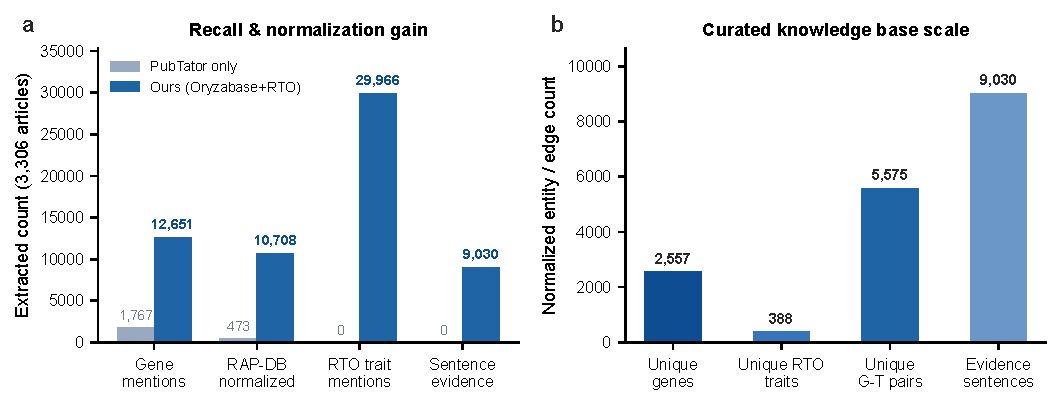
\includegraphics[width=\textwidth]{figure/fig3_pipeline_ablation.pdf}
    \caption{实体识别与归一化消融及知识库规模。(a) 通用 PubTator 与本文双词典流水线的数量对比；(b) 五重消歧后的知识网络规模。}
    \label{fig:ablation}
  \end{minipage}\hfill
  \begin{minipage}[t]{0.485\textwidth}
    \centering
    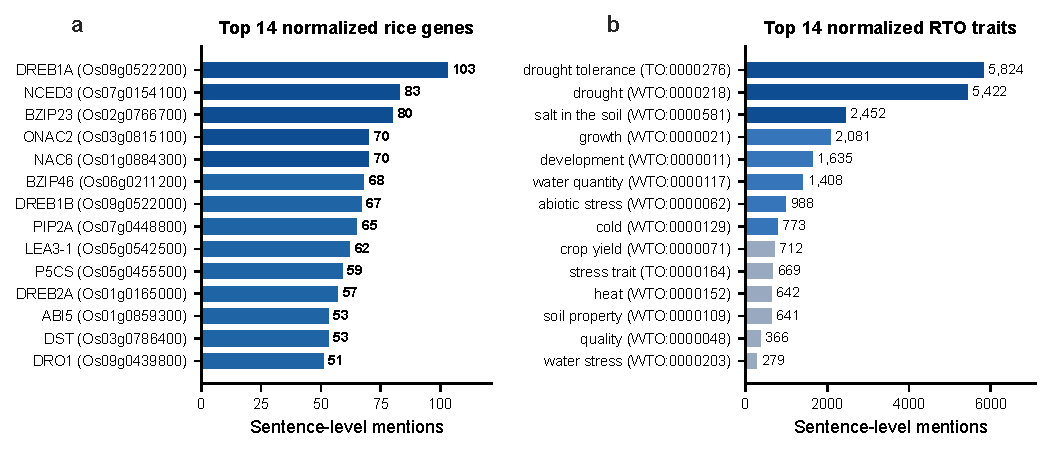
\includegraphics[width=\textwidth]{figure/fig4_top_genes_traits.pdf}
    \caption{归一化后高频抗旱基因与 RTO 性状。(a) Top14 基因（标注 RAP ID）；(b) Top14 性状。}
    \label{fig:top_entities}
  \end{minipage}
\end{figure*}

\subsection{实体归一化与共现基线}
全语料共定位 42,617 处实体提及：RAP 归一化水稻基因 10,708 处、RTO 性状 29,966 处，另有 1,943 处 PubTator-only 非水稻基因用于负向掩码。相比通用 PubTator 的 473 处 RAP 映射，基因归一化提升 22.6 倍，并补齐了 PubTator 完全缺失的性状维度（图~\ref{fig:ablation}a）。水稻-only 候选共现为 7,868 条，连接 1,344 个基因、190 个性状、4,678 个唯一基因-性状对（图~\ref{fig:ablation}b）。

表~\ref{tab:top_genes} 给出 Top10 基因及其别名汇聚实证。以 \texttt{ONAC2}（\texttt{Os03g0815100}）为例，文献中 \texttt{SNAC1}（51 次）、\texttt{OsNAC9}（12 次）、\texttt{OsSNAC1}（6 次）与 \texttt{ONAC2}（1 次）被统一收敛；\texttt{DREB1A} 则混用 \texttt{DREB1A}、\texttt{OsDREB1A} 与拟南芥同源命名 \texttt{CBF3}。若不归一化，这些证据将被割裂为互不相干的碎片。Top14 基因（\texttt{DREB1A}、\texttt{NCED3}、\texttt{BZIP23}、\texttt{ONAC2}、\texttt{NAC6}、\texttt{BZIP46}、\texttt{DREB1B}、\texttt{PIP2A}、\texttt{LEA3-1}、\texttt{P5CS}、\texttt{DREB2A}、\texttt{ABI5}、\texttt{DST}、\texttt{DRO1}）均为植物分子生物学界公认的水稻抗旱骨干基因。

\begin{table*}[t]
  \centering
  \fontsize{6.9pt}{7.9pt}\selectfont
  \renewcommand{\arraystretch}{0.76}
  \setlength{\tabcolsep}{3.2pt}
  \caption{Top10 水稻抗旱基因的别名汇聚与 RAP-DB 归一化}
  \label{tab:top_genes}
  \begin{tabularx}{\textwidth}{c l l c p{6.4cm} X}
    \toprule
    排名 & 标准符号 & RAP-DB & 提及数 & 语料中自动归并的异构写法（频次） & 基因全称与抗旱机制 \\
    \midrule
    1 & \textbf{DREB1A} & \texttt{Os09g0522200} & 103 & \texttt{DREB1A} (37), \texttt{OsDREB1A} (31), \texttt{CBF3} (24), \texttt{DREB1a} (9), \texttt{Cbf3} (2) & AP2/ERF 转录因子，结合 DRE 元件激活抗逆基因 \\
    2 & \textbf{NCED3} & \texttt{Os07g0154100} & 83 & \texttt{OsNCED3} (36), \texttt{OsNCED4} (27), \texttt{NCED4} (10), \texttt{NCED3} (8) & ABA 生物合成关键限速酶 \\
    3 & \textbf{BZIP23} & \texttt{Os02g0766700} & 80 & \texttt{OsbZIP23} (70), \texttt{osbZIP23} (4), \texttt{OsZIP23} (2), \texttt{OsAREB2} (2) & 华农克隆的 ABA 敏感型 bZIP 因子 \\
    4 & \textbf{ONAC2} & \texttt{Os03g0815100} & 70 & \texttt{SNAC1} (51), \texttt{OsNAC9} (12), \texttt{OsSNAC1} (6), \texttt{ONAC2} (1) & 华农明星基因 SNAC1，诱导气孔关闭、改良根系 \\
    5 & \textbf{NAC6} & \texttt{Os01g0884300} & 70 & \texttt{OsNAC6} (40), \texttt{OsNAC2} (14), \texttt{SNAC2} (10), \texttt{NAC6} (3) & NAC 转录因子，激活过氧化物酶与根系通路 \\
    6 & \textbf{BZIP46} & \texttt{Os06g0211200} & 68 & \texttt{OsbZIP46} (41), \texttt{OsABF2} (8), \texttt{OsbZIP46CA1} (7), \texttt{ABF3} (5) & AREB/ABF 亚家族，正调控抗旱响应 \\
    7 & \textbf{DREB1B} & \texttt{Os09g0522000} & 67 & \texttt{OsDREB1B} (38), \texttt{DREB1B} (12), \texttt{CBF1} (9), \texttt{OsDREB1C} (7) & 逆境诱导型 DREB，提升脱水耐受性 \\
    8 & \textbf{PIP2A} & \texttt{Os07g0448800} & 65 & \texttt{OsPIP2} (49), \texttt{PIP2} (12), \texttt{OsPIP2a} (3), \texttt{OsPIP2-1} (1) & 质膜水通道蛋白，调控根系水力导度 \\
    9 & \textbf{LEA3-1} & \texttt{Os05g0542500} & 62 & \texttt{OsLEA3} (34), \texttt{OsLEA3-1} (11), \texttt{LEA3} (7), \texttt{Lea3} (4) & 胚胎晚期丰富蛋白，保障大田干旱下结实率 \\
    10 & \textbf{P5CS} & \texttt{Os05g0455500} & 59 & \texttt{P5CS} (33), \texttt{OsP5CS} (12), \texttt{OsP5CS1} (9), \texttt{P5CS1} (5) & 脯氨酸合成限速酶，维持细胞渗透势 \\
    \bottomrule
  \end{tabularx}
\end{table*}

\subsection{SDP 因果抽取与人工审计}
在 7,868 条候选上，SDP 保留 884 条因果调控关系（575 正、150 负、159 中性）与 1,379 条 association；5,489 条因缺少基因→性状论元方向被排除，48 条因 \texttt{respectively} 错配被排除，35 条为否定/无效应，33 条无依存路径（图~\ref{fig:sdp}a--b）。884 条因果覆盖 385 个基因、693 个唯一基因-性状对；正/负极性比为 3.8:1，与抗旱基因以正向调控为主的生物学先验一致（图~\ref{fig:sdp}c）。

\begin{figure*}[t]
  \centering
  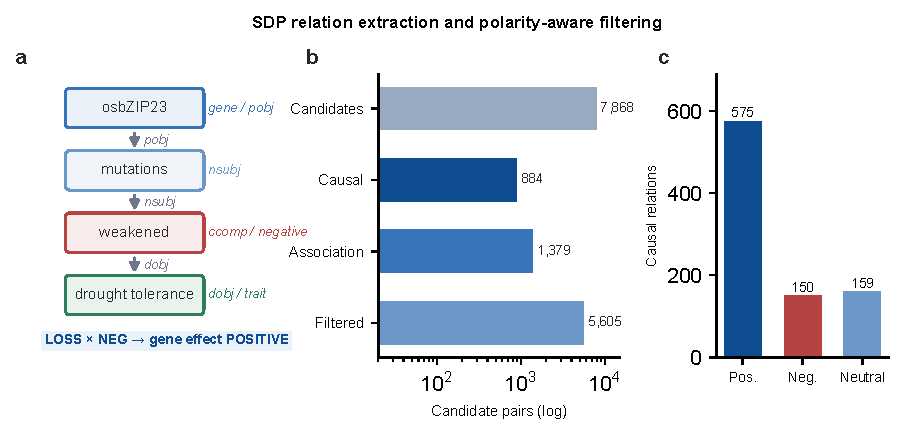
\includegraphics[width=0.66\textwidth]{figure/fig5_sdp_framework.pdf}
  \caption{SDP 因果抽取框架。(a) \texttt{osbZIP23} 突变降低 \texttt{drought tolerance} 的路径；loss-of-function 构建与 negative 谓词双重取反，得到基因正向调控；(b) 7,868 条候选的过滤漏斗；(c) 884 条因果关系的极性构成。}
  \label{fig:sdp}
\end{figure*}

为量化抽取质量，按“SDP 因果层 / 非因果层”分层随机抽取 100 条候选（各 50 条），由作者逐条标注为正向、负向、方向未知的因果或非因果。审计定义：句子必须明确表明该基因（或其过表达/敲除/突变）影响该性状；仅共现、关联、表达相关、调控其他性状、否定或无效应均记为负例。结果如图~\ref{fig:eval}(a)：SDP precision 86.0\%（95\% CI 73.8--93.0），共现基线加权 precision 34.5\%；按分层外推，SDP recall 28.0\%、F1 42.2\%，极性准确率 88.2\%（34 条可判极性样本）。Recall 偏低是因为大量真实关系以 \texttt{showed enhanced tolerance}、\texttt{is required for}、\texttt{mutant with increased tolerance} 等名词语义表达，规则尚未覆盖；这些案例被保留在 association 层，供后续模型召回。

\begin{figure*}[t]
  \centering
  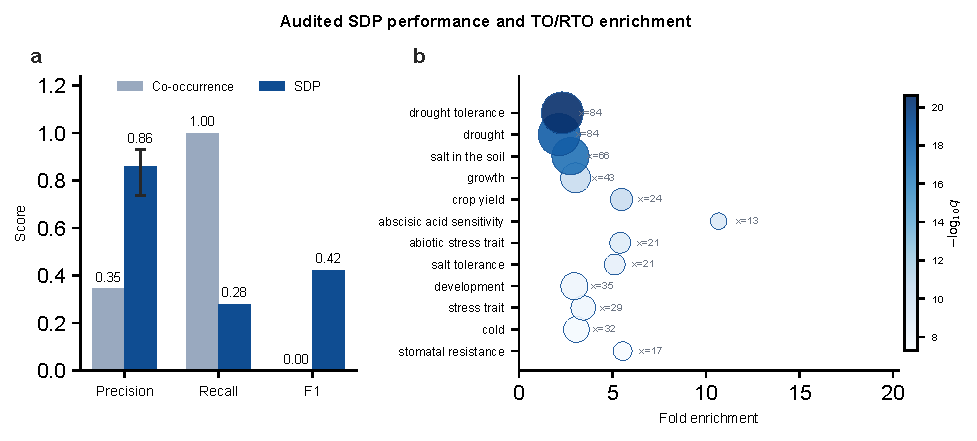
\includegraphics[width=0.66\textwidth]{figure/fig6_evaluation_enrichment.pdf}
  \caption{(a) 100 条分层审计的 Precision/Recall/F1：共现基线 vs.\ SDP；(b) Top100 SDP 因果基因集的 TO/RTO 富集气泡图（气泡大小 $=x$，颜色 $=-\log_{10}q$）。}
  \label{fig:eval}
\end{figure*}

表~\ref{tab:audit} 给出 6 条代表性审计案例。正确案例覆盖直接调控、loss-of-function 反转与 \texttt{respectively} 对齐；错误案例暴露三类残余问题：实体与性状词同形（\texttt{D1}/RGA）、否定/间接调控被误判、以及多分句谓词选择错误。与阶段二的两个经典错误（\texttt{SAMs} 与 \texttt{SAMS1} 同形、\texttt{OsBIHD1} 受 \texttt{respectively} 约束）相比，SDP 已消除并列错配（48 条被显式排除），但组织缩写与跨分句论元仍是主要误差源。

\begin{table*}[t]
  \centering
  \fontsize{6.7pt}{7.7pt}\selectfont
  \renewcommand{\arraystretch}{0.74}
  \setlength{\tabcolsep}{3.0pt}
  \caption{SDP 人工审计的代表性正确案例与错误案例}
  \label{tab:audit}
  \begin{tabularx}{\textwidth}{c p{2.6cm} p{2.6cm} p{1.4cm} X}
    \toprule
    ID & 基因 / 性状 & SDP 输出 & Gold & 诊断与原文（节选） \\
    \midrule
    A02 & SST / salt & negative & $-1$ & 正确：\textit{OsSPL10 negatively regulates salt and drought stress tolerance} \\
    A46 & PRX130 / drought tolerance & positive & $+1$ & 正确：knockout 降低 tolerance，loss-of-function 反转 \\
    A36 & BHLH148 / drought tolerance & regulation & reg & 正确：\texttt{respectively} 将 bHLH148 对齐到 drought \\
    A04 & PFA-DSP1 / drought tolerance & positive & $-1$ & 错误：overexpression 增加 drought sensitivity，谓词 \texttt{increased} 未结合宾语语义 \\
    A07 & GSTU17 / drought tolerance & negative & $+1$ & 错误：knockout 降低 tolerance，反转规则未命中 \\
    A01 & D1 / water quantity & regulation & 0 & 错误：句子主语是 root growth angle，未出现 D1，实体错配 \\
    \bottomrule
  \end{tabularx}
\end{table*}

\subsection{TO/RTO 富集与 RiceMind 注释缺口}
以 SDP 因果证据排序的 Top100 基因为查询集，在 2,218 个背景基因、272 个 TO/RTO 条目上执行超几何富集。共 151 个条目被命中，53 个达到 $q<0.05$；图~\ref{fig:eval}(b) 展示 Top12。\texttt{drought tolerance}（$x=84$，fold 2.32）、\texttt{drought}（84，2.15）、\texttt{salt in the soil}（66，2.76）居前，\texttt{abscisic acid sensitivity}（13，10.68）、\texttt{grain size}（8，8.87）、\texttt{stomatal resistance}（17，5.54）显示强富集；ABA 敏感性与气孔抗性正是抗旱网络的核心枢纽，说明 SDP 因果基因集在功能层面高度内聚。14 个核心基因的富集更强（68 个显著条目，\texttt{drought tolerance} $x=14/14$），但该集合本身由高频抗旱文献选出，存在选择偏倚，故本文以 Top100 结果作为主证据。

RiceMind 交叉验证显示，Top100 中 99 个可检索到标准 RAP 记录（99\%），85 个具有 stress/tolerance 注释，但仅 13 个在 \texttt{annotation} 中明确出现 drought/water deficit。这一“一般逆境注释丰富、干旱特异注释稀疏”的落差，正是文献挖掘可以补足的价值。按“$\ge3$ 个唯一对且无 stress 注释”筛选，得到 13 个注释缺口候选；表~\ref{tab:novel} 列出前 5 个。需要强调，这些并非全新基因，而是 RiceMind 当前注释未覆盖、但 SDP 文献证据支持其抗逆关联的候选，需人工审编与实验验证。基因-性状网络共 457 个节点、693 条边；图~\ref{fig:network} 展示 Top10 基因与 Top8 性状的二分结构，\texttt{DSR2}、\texttt{ONAC2}、\texttt{WOX11}、\texttt{HDA704} 等处于高连接度位置。

\begin{table}[t]
  \centering
  \fontsize{6.8pt}{7.8pt}\selectfont
  \renewcommand{\arraystretch}{0.78}
  \setlength{\tabcolsep}{2.6pt}
  \caption{RiceMind 抗逆注释缺口候选（Top5）}
  \label{tab:novel}
  \begin{tabularx}{\columnwidth}{c l l c X}
    \toprule
    排名 & 基因 & RAP ID & 唯一对 & 主要 SDP 性状（频次） \\
    \midrule
    1 & DRAP1 & \texttt{Os11g0544700} & 5 & drought tolerance (2), salt tolerance (1) \\
    2 & ANN1 & \texttt{Os01g0497400} & 4 & stress trait (1), abiotic stress (1), heat (1) \\
    3 & CALA & \texttt{Os05g0491100} & 4 & abiotic stress (1), heat (1), growth (1) \\
    4 & BHC & \texttt{Os04g0624500} & 4 & stomatal opening (2), salt (2) \\
    5 & -- & \texttt{Os01g0178600} & 4 & drought (1), drought tolerance (1), cold (1) \\
    \bottomrule
  \end{tabularx}
\end{table}

\begin{figure}[t]
  \centering
  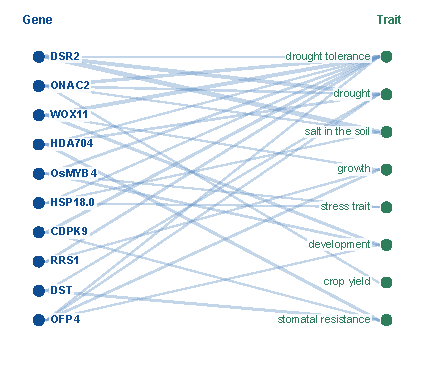
\includegraphics[width=0.95\columnwidth]{figure/fig7_gene_trait_network.pdf}
  \caption{SDP 因果网络的二分结构（Top10 基因 × Top8 性状；边宽为证据数）。}
  \label{fig:network}
\end{figure}

\section{讨论}
\subsection{结果意味着什么}
本文的三点发现具有方法学意义。第一，检索式与词汇计量应互相校验：TF-IDF 证明 \texttt{drought stress} 比 \texttt{drought tolerance} 多覆盖 41.9\% 文献，窄口径检索会系统性漏检。第二，农业实体归一化必须“词典+规则+负向掩码”协同：Oryzabase 将基因归一化提升 22.6 倍，但 \texttt{ABA}、\texttt{ha-1}、\texttt{Apo} 等冲突必须显式拦截。第三，共现与因果应分层：SDP 将 precision 从 34.5\% 提升到 86.0\%，但 recall 仅 28.0\%；二者不是替代关系，而是“高精度因果层 + 高覆盖 association 层”的互补结构。

\subsection{局限性与真实错误}
（1）实体同形：组织缩写 \texttt{SAMs} 与基因 \texttt{SAMS1}、根生长角 \texttt{RGA} 与基因 \texttt{D1} 仍会被静态词典误配；表~\ref{tab:audit} 的 A01 即典型。（2）谓词/极性：多分句句中谓词可能选错（A04），部分 loss-of-function 表达（\texttt{knockout} 以外的 \texttt{CRISPR-edited variants}）未触发反转（A07）。（3）覆盖：SDP 规则偏保守，\texttt{showed enhanced tolerance}、\texttt{is required for development}、\texttt{mutant with increased tolerance} 等名词语义尚未覆盖，recall 偏低。（4）数据：5 篇 2026 年新文献未被 PubTator 索引；RiceMind 注释以人工审编为主，存在滞后。

\subsection{下一步}
短期将把轻动词+评价形容词、\texttt{required for}、\texttt{positive regulator of} 等模式纳入规则，并用依存树上的否定/并列约束做后处理；中期引入 PubMedBERT 或指令微调模型做小样本关系分类，以规则输出为弱监督；长期对接 RiceMind 多组学与 GO 富集，构建“文献证据--表达--变异--表型”四层知识图谱，并对表~\ref{tab:novel} 的候选做实验验证。

\section{结论}
本文完成了从 PubMed 语料到水稻抗旱基因-性状知识图谱的端到端流水线：3,306 篇全文、795,401 词元、102,860 条基因别名、3,904 条性状同义词、7,868 条水稻候选对；SDP 抽取 884 条因果调控关系与 1,379 条 association，人工审计 precision 86.0\%、极性准确率 88.2\%；TO/RTO 富集 53 个显著条目，RiceMind 交叉验证暴露 13 个注释缺口候选。该流水线为作物抗逆知识发现提供了可追溯、可复现的语料与关系底座。

\section*{数据与代码可用性}
本文全部脚本与中间结果已随论文归档：\texttt{scripts/01}--\texttt{06} 覆盖 PubMed/PubTator 下载、TTR/TF-IDF、Oryzabase/RTO 词典构建、句子级证据抽取与图表生成；\texttt{scripts/07}--\texttt{11} 覆盖 SDP 抽取、100 条分层审计、TO/RTO 富集、RiceMind 交叉验证与阶段三/四图表。关键输出包括 \texttt{rice\_drought\_sentence\_evidence.tsv}（7,868 条候选）、\texttt{sdp\_relations.tsv}（884 条因果 + 1,379 条 association）、\texttt{sdp\_audit\_100.csv} 与 \texttt{sdp\_audit\_labels.json}（人工标签）、\texttt{part4\_enrichment\_summary.json} 与 \texttt{part4\_novel\_targets.csv}。所有字符偏移均通过 \texttt{text[b:e]==mention} 断言，随机种子、样本分层与 BH 校正参数在脚本中固定。代码仓库：\url{https://github.com/ZimingADR/BioNLP}。

\section*{致谢}
感谢华中农业大学《生物文本挖掘与知识发现》课程与夏静波老师的指导；感谢 Oryzabase、RAP-DB、RiceMind 与 RTO 团队开放数据与接口。本文实验由作者设计并复核，Agent 仅用于代码实现、数据整理与文字起草。

\bibliographystyle{IEEEtran}
\bibliography{reference}

\end{document}